% Created 2016-02-09 Tue 21:18
\documentclass[11pt]{article}
\usepackage[utf8]{inputenc}
\usepackage[T1]{fontenc}
\usepackage{fixltx2e}
\usepackage{graphicx}
\usepackage{grffile}
\usepackage{longtable}
\usepackage{wrapfig}
\usepackage{rotating}
\usepackage[normalem]{ulem}
\usepackage{amsmath}
\usepackage{textcomp}
\usepackage{amssymb}
\usepackage{capt-of}
\usepackage{hyperref}
\usepackage{setspace}
\doublespacing
\usepackage[margin=2.54cm]{geometry}
\author{Jake Brawer}
\date{\today}
\title{Thesis Manuscript}
\hypersetup{
 pdfauthor={Jake Brawer},
 pdftitle={Thesis Manuscript},
 pdfkeywords={},
 pdfsubject={},
 pdfcreator={Emacs 24.5.1 (Org mode 8.3.1)}, 
 pdflang={English}}
\begin{document}

\maketitle

\section*{Chapter 1: Literature Review}
\label{sec:orgheadline13}
I think the best approach for this thesis is to frame it in a larger discussion on the nature of intelligence. I begin with a brief historical overview/discussion of the shift in the prevailing view of the mind as a symbol manipulator, to an embodied and embedded system, as seen primarily through the GOFAI/BBAI debate. I think this leads naturally into a discussion of evolutionary robotics as a means of exploiting brain-body-environment coupling to autonomously design robots. From here I can discuss evolution and G->P mapping. Specifically how adaptive, noncontrol related morphologies and structures can be considered a form of intelligence. Also discuss G->P maps and evolvability, and how modeling aspects o evolvable G->P maps (e.g. modularity, robustness,and especially development etc.) Can lead to innovative robot designs. Finally, I discuss our experiments, the goal of which is evaluate the efficacy of incorporating ontogenetic processes into an evolutionary robotics context.
\subsection*{Embodied Intelligence/Robotics}
\label{sec:orgheadline3}

\subsubsection*{GOFAI vs. BBAI}
\label{sec:orgheadline1}
\begin{itemize}
\item Anderson, M. L. (2003). Embodied cognition: A field guide. Artificial intelligence, 149(1), 91-130.
\item Alonso, E. (2002). AI and agents: state of the art. AI Magazine, 23(3), 25.
\begin{itemize}
\item Discusses GOFAI's limitations in uncertain environments
\begin{itemize}
\item The "point" of robotics is to design agents that can negotiate uncertainty without human intervention 
\begin{itemize}
\item The goal then is to design robust learning algorithms
\begin{itemize}
\item \textbf{My note:} Rather than design one a priori, we can design systems sensitive to evolution so that they may evolve their own learning strategies.
\end{itemize}
\end{itemize}
\end{itemize}
\end{itemize}
\end{itemize}
\subsubsection*{How bodily/developmental constraints shape/produce intelligence}
\label{sec:orgheadline2}
\begin{itemize}
\item Chiel, H. J., \& Beer, R. D. (1997). The brain has a body: adaptive behavior emerges from interactions of nervous system, body and environment. Trends in neurosciences, 20(12), 553-557.
\begin{itemize}
\item Bodies constrain and shape intelligence
\begin{itemize}
\item "The close matching between the nervous system and the periphery creates both constraints and opportunities for the nervous system.
\item This ties into the how the Braitenbot evolves. 
\begin{itemize}
\item The topology of the pins constrain the development of the threads and thus constrain intelligence
\end{itemize}
\end{itemize}
\end{itemize}
\end{itemize}
\subsection*{Why evolutionary robotics? What are the benefits?}
\label{sec:orgheadline5}
\Harvey, I., Di Paolo, E., Wood, R., Quinn, M., \& Tuci, E. (2005). Evolutionary robotics: A new scientific tool for studying cognition.  Artificial life, 11(1-2), 79-98.
\begin{itemize}
\item Provides a brief historical overview of evolutionary robotics
\end{itemize}
\subsubsection*{Challenges in evolving robots}
\label{sec:orgheadline4}
\begin{itemize}
\item Matarić, M., \& Cliff, D. (1996). Challenges in evolving controllers for physical robots. Robotics and autonomous systems, 19(1), 67-83.
\item Watson, R. A., Ficici, S. G., \& Pollack, J. B. (2002). Embodied evolution: Distributing an evolutionary algorithm in a population of robots. Robotics and Autonomous Systems, 39(1), 1-18.
\begin{itemize}
\item Discusses the benefits of evolving/testing multiple robots simultaneously
\begin{itemize}
\item Is very fast
\item Takes physical load off a single robot.
\end{itemize}
\end{itemize}
\end{itemize}
\subsection*{G-P mapping as the manufactory for organisms/robots}
\label{sec:orgheadline12}

\subsubsection*{What is a G->P Map?}
\label{sec:orgheadline6}

Source: Pigliucci, M. (2010). Genotype–phenotype mapping and the end of the ‘genes as blueprint’metaphor. Philosophical Transactions of the Royal Society B: Biological Sciences, 365(1540), 557-566.
\begin{itemize}
\item Provides a great explanation of G->P mapping
\item Discusses genetic-ontogenetic co-constitution of phenotype
\end{itemize}


\subsubsection*{Evolvability}
\label{sec:orgheadline10}
\begin{itemize}
\item Variation vs. Variability determine evolvability
\label{sec:orgheadline7}

Source: Pigliucci, M. (2008). Is evolvability evolvable?. Nature Reviews Genetics, 9(1), 75-82.
\begin{itemize}
\item \textbf{Variation}:  "Measure of realized differences within a population"
\item \textbf{Variability}: "The propensity of a character to vary" (whether or not they actually do)
\end{itemize}
Variability is depends on G->P map (How it produces phenotype through developmental interactions
with the environment.

"Evolvability is the propensity to vary that is afforded by the genetic architecture"
\begin{itemize}
\item emphasizes the relevance of genetic networks over individual genes.
\begin{itemize}
\item And therefore emphasizes developmental affects on the phenotype.
\end{itemize}
\end{itemize}
\item Modularity (Neccessary for highly evolved systems)
\label{sec:orgheadline8}
Bongard, J. C., \& Pfeifer, R. (2001). Repeated structure and dissociation of genotypic and phenotypic complexity in artificial ontogeny. In Proceedings of the Genetic and Evolutionary Computation Conference (Vol. 829836).
\item Robustness
\label{sec:orgheadline9}

Development systems are robust when they can accrue  genetic variants (via mutation) without phenotypic or fitness effects
\begin{itemize}
\item robustness can be selected for
\end{itemize}
\end{itemize}
\subsubsection*{Limitations of 1-1 mapping/ Importance of Ontogeny in G-P maps}
\label{sec:orgheadline11}

F. Delleart, and R. D. Beer (1994). Toward an evolvable
model of development for autonomous agent synthesis. In
Artificial Life IV, 246–257. MIT Press
\begin{itemize}
\item Discusses the artificial nature of 1-1 mappings
\begin{itemize}
\item Morphologies are the result of growth \emph{processes}, which are ontogentic in nature
\end{itemize}
\item Discusses Drawbacks
\begin{itemize}
\item The designs to be explored are essentially limited by the chosen architecture,because of the fixed dimensionality.
\item Scales badly for large networks
\item Bilateral symmetry difficult in 1-1 mapping
\end{itemize}
\end{itemize}
\section*{Chapter 2: Materials and Methods}
\label{sec:orgheadline21}
\subsection*{Materials}
\label{sec:orgheadline20}
\subsubsection*{The Braitenbot}
\label{sec:orgheadline14}

The Ana Bbot from JoHuCo (Braitenbot) is a battery-powered vehicle inspired by the writings of Valentino Braitenberg. In addition to two posterior wheels powered by a differential drive, the Braitenbot utilizes an anterior unpowered catser wheel to maintain balance. The user interface of the Braitenbot is implemented by its open circuit board, located at the top of the robot (Fig 1). The circuit board is essentially an analog computer, with modifiable wire connections mediating the analog signals between components. These wires connect to exposed headers, or ‘pins’ with each component having a corresponding group of functionally equivalent pins (pin group). Components include four sensors, left and right IR sensors (labelled RL and RR on the circuit board, see Fig. 1) and left 
and right photosensors (PL and PR respectively); six neurons; and two motors, with connections that allow left and right forward movement
 (FL and FR respectively) and left and right backward movement (BL and BR respectively). 

The connection of the sensors to the circuit can be easily changed as part of the programming that occurs in hardware.  The six neurons
have excitatory (E1-E6) and inhibitory (I1-I6) pin groups, which allow signals coming from sensors or other neurons to act as excitatory
 and inhibitory input to the target neuron. The neuron sums these inputs and outputs this sum to a pin group (N1-N6). In parallel, 
the neuron takes the sum and thresholds a response to a different pin group (T3-T6). Sensors or neurons may connect directly to the motors and their voltages are converted into commands for the wheels. 

\subsubsection*{The Code}
\label{sec:orgheadline19}

\begin{itemize}
\item Bases
\label{sec:orgheadline15}

A Braitenbot’s genome is a list data structure (with indices) containing objects called “Bases” (the size of the list is easily modifiable in the source code). A Base is an object containing two values, a “char” value and a “hotspot” value, both binary, but interpreted by the decoder differently.  A char is analogous to a nucleobase; it is used by the decoder to help create the phenotype (see Decoder section) but does not by itself code for a trait. There is an equal chance for any given Base that its char will be a 1 or a 0.  A hotspot value of 1 denotes a recombination hotspot in the genome. That is, the point at which the decoder stops copying Bases from a parent’s genome to an offspring’s (see below). Currently there is a 1/1000 chance that the hotspot value for a given Base will be 1 (though this probability is easily modifiable).

\item Genome
\label{sec:orgheadline16}

During sexual reproduction, the genomes of two parents are recombined to form a novel genome for their offspring. One individual is chosen at random to be the “dominant” parent. This means that only the dominant’s hotspots are used to direct recombination. The reproduction algorithm first walks incrementally through the dominant’s genome, copying Bases to the offspring’s genome until a hotspot value of 1 is encountered. At this point, it will start copying Bases from the other parent genome starting at the corresponding locus. Everytime the algorithm encounters a hotspot value of 1, it switches to the other parent's genome. 

How often an individual reproduces, and with whom the individual reproduces, is partially dependent on fitness. The reproduction algorithm ranks individuals based on experimental performance; The two highest performing individuals are placed in the highest rank, the next two highest performing individuals in the second highest rank etc. until all individuals hav been ranked. The crossing algorithm begins by randomly crossing individuals with the highest rank. Once an individual is crossed, they are placed in the next highest rank, and can be crossed again, unless they were in the lowest rank, in which case they are removed from the gene pool. Crossing terminates when all individuals in the lowest rank have been crossed. Under this scheme, given an population of ten individuals, the subsequent population is guaranteed to contain 10 offspring, although the parentage of the offspring is partially under the control of random processes.
\item Decoder And Threads
\label{sec:orgheadline17}

At the most abstract level, the Braitenbot’s phenotype (i.e., those traits constructed by the genome) could be thought to consist of discrete “neuromodules” we denote as “threads.” A thread can be conceived of as a network of continuous wire connections that connect components of the Braitenbot in a feedforward fashion (although it is not out of the realm of possibility to get threads that loop on the same pin group, or vacillate between two). Threads are “grown” simultaneously, wire by wire, in a round-robin fashion starting from the thread coded by the leftmost part of the genome. If two or more threads collide at a single pin, the one that grew to the pin first claims the pin and the others terminate at the point of contention (this may imply that there is pressure on genes to be as far left, meaning first in order of expression, on the genome as possible).  A thread is primarily constructed by the Decoder, which translates the genome (using the char values) into wiring instructions.  The Decoder treats the genome as if it were composed of 4-bit binary numerals, and translates these 4-bit numerals into decimal numbers. That is, the Decoder analyzes the char value of the Bases four at a time, and uses these values to construct one decimal digit (theoretically a 4-bit binary numeral can be as large as the decimal number 16 however, we arbitrarily decided that any 4-bit string > 9 is not translated into a number and the thread ends there).  Four-bit strings > 9 could potentially be used as stop and/or stop codons if necessary.

These numbers are used to specify the start and end points for the wire connections that constitute a given thread. All the possible connection points on the Braitenbot are represented by elements in a matrix, with each element denoted by a specific x-y coordinate. The Decoder uses the sequence of decoded decimal numbers as movement instructions for an “automaton” that traverses the matrix. The automaton can “jump” from element to element, and its resulting path through the matrix is interpreted as wiring instructions. Therefore, a single gene in this model could be considered to be the Bases comprising a single thread.

The first two numbers are used to determine the starting coordinates of the automaton, and thus the origin point of a thread. The next number decides the direction (of 8 possible directions) of the jump, and the last number the distance of the jump. If a thread contains more than one wire, the origin of the first wire will be the adjacent free pin in the pin group of the terminus of the previous wire connection. It is possible for the automaton to jump out of the bounds of the matrix, as well as jump to an element that does not correspond to a pin on the Braitenbot (by necessity there are more elements in the matrix than pins on the Braitenbot). If either of these two cases occur, the thread terminates at the previous wire connection (if there was one).  As it stands, the maximum number of wires in a thread is arbitrarily set, and thus the demarcation between Bases corresponding to a particular thread are as well. Ideally, we will implement start and stop codons, which signify the start and end of a thread respectively. This would allow for more dynamic thread sizes, and would also enhance bio-plausibility.

For pragmatic purposes, we impose a number of phenotypic “checks” on the algorithm that generates an initial population of organisms to test. These checks ensure that there is at least one thread in each individual that has a sensor to motor connection, meaning that every individual will be able to locomote in some fashion initially.
`
\item The Non-Developmental Model
\label{sec:orgheadline18}

The non-developmental model is the baseline by which we will evaluate the efficacy of the developmental model. We typify development in the experimental model by allowing the genomic expression of a gene to be modulated by its genomic context, as well as having the topology of the Braitenbot constrain thread 'growth.' To this end, The non-developmental model implementation-wise is identical to the developmental model aside from one key differences: Collisions are not allowed. This means that if two or more threads happen to occupy the same space, an adjacent pin in the same pin group will be assimilated by the thread, and both threads will continue developing as if no collision had a occured. The end result is that if a coding region is present in a genome, it has to be expressed, irrespective of its genomic context.
\end{itemize}

\section*{Chapter 3: Simulation and Experiment}
\label{sec:orgheadline38}
\subsection*{Simulations}
\label{sec:orgheadline32}

We ran a number of evolutionary trials in simulation to 1) determine if our model facilitated adaptive evolution, and 2) to empirically determine genomic parameters that would support adaptive evolution. Here we selected for genomes that produced the highest number of "active threads," i.e. threads that produced at least one viable wire connection. Given that this method of selection did not require actual robots to be wired, it afforded the opportunity to run multiple evolutionary trials and multiple different populations in a relatively short amount of time. 

We ran multiple populations altering different genomic parameters (e.g. genome length, crossover point number, coding region length, etc.) for each population, and compared the results. Each population was run three times, and generational fitness averages were themselves averaged across the three runs. The results are as follows:

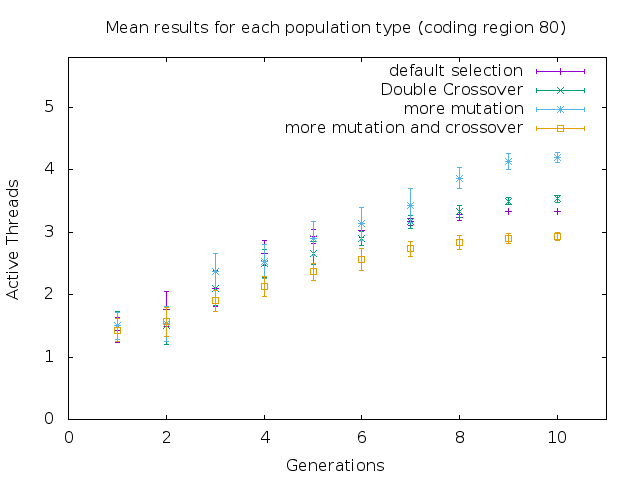
\includegraphics[width=.9\linewidth]{population-comparison-80-1.png}

\subsubsection*{Graph key}
\label{sec:orgheadline26}

\begin{itemize}
\item Default
\label{sec:orgheadline22}

\begin{itemize}
\item Genome len: 560
\item Num Crossover points: 2
\item Mutation rate: 20000
\item Unrestricted crossover: True
\item coding region len: 80
\end{itemize}

\item Double Crossover
\label{sec:orgheadline23}

\begin{itemize}
\item Genome len: 560
\item Num Crossover points: 4
\item Mutation rate: 20000
\item Unrestricted crossover: True
\item coding region len: 80
\end{itemize}

\item More Mutation
\label{sec:orgheadline24}

\begin{itemize}
\item Genome len: 560
\item Num Crossover points: 2
\item Mutation rate: 2000
\item Unrestricted crossover: True
\item coding region len: 80
\end{itemize}


\item More Mutation And Double Crossover
\label{sec:orgheadline25}

\begin{itemize}
\item Genome len: 560
\item Num Crossover points: 4
\item Mutation rate: 2000
\item Unrestricted crossover: True
\item coding region len: 80
\end{itemize}

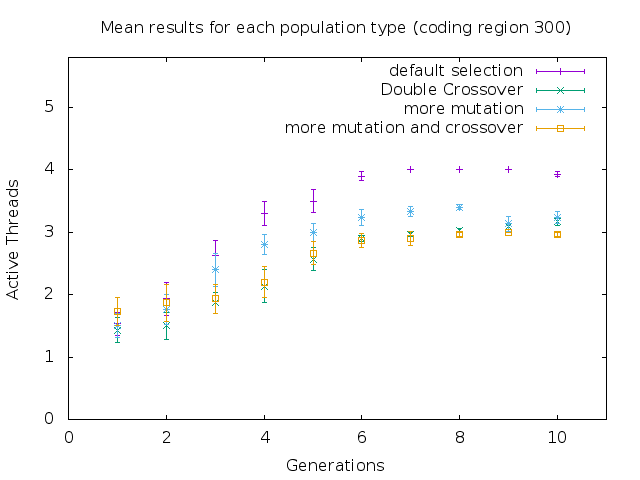
\includegraphics[width=.9\linewidth]{population-comparison-300.png}
\end{itemize}


\subsubsection*{Graph key}
\label{sec:orgheadline31}

\begin{itemize}
\item Default
\label{sec:orgheadline27}

\begin{itemize}
\item Genome len: 2100
\item Num Crossover points: 2
\item Mutation rate: 20000
\item Unrestricted crossover: True
\item coding region len: 300
\end{itemize}

\item Double Crossover
\label{sec:orgheadline28}

\begin{itemize}
\item Genome len: 2100
\item Num Crossover points: 4
\item Mutation rate: 20000
\item Unrestricted crossover: True
\item coding region len: 300
\end{itemize}

\item More Mutation
\label{sec:orgheadline29}

\begin{itemize}
\item Genome len: 2100
\item Num Crossover points: 2
\item Mutation rate: 2000
\item Unrestricted crossover: True
\item coding region len: 300
\end{itemize}


\item More Mutation And Double Crossover
\label{sec:orgheadline30}
\begin{itemize}
\item Genome len: 2100
\item Num Crossover points: 4
\item Mutation rate: 2000
\item Unrestricted crossover: True
\item coding region len: 300
\end{itemize}


Based on these results we decided that all populations would use the "more mutation" parameters with a coding region length of 80.
\end{itemize}
\subsection*{Experiment}
\label{sec:orgheadline37}
\subsubsection*{Overview}
\label{sec:orgheadline36}

The goal of this thesis is to evaluate the efficacy and viability of incorporating developmental processes into an evolutionary robotic system. To this end we devised a comparative evolutionary experiment consisting of multiple population, with the goal of evolving individuals competent in both phototaxis and obstacle avoidance. 

\begin{itemize}
\item Experimental Groups
\label{sec:orgheadline33}

Two experimental populations were evolved. Each population was run for ten generations, with each generation containing ten individuals. The two experimental groups differed in the architecture they implemented, i.e. the developmental or non-developmental architecture. Additionally two control populations were evolved. The control populations also implemented one of the aforementioned architecture, although control individuals were selected for randomly, rather than as a function of their fitness as with the experimental populations.

\item Experimental design
\label{sec:orgheadline35}
\begin{itemize}
\item Exact specifications and figures will be placed here when finalized.
\label{sec:orgheadline34}
\end{itemize}
\end{itemize}
\section*{Chapter 4: Results and Discussion}
\label{sec:orgheadline41}
\subsection*{Results and analysis}
\label{sec:orgheadline39}

\begin{itemize}
\item Report relevant statistics
In order to evaluate the efficacy of a developmental-evolutionary system, we might want to compare the populations along a few different metrics, including:
\begin{itemize}
\item Mean amount of light collected (fitness)
\item Generation at which peak fitness was reached (search efficiency)
\item Mean number of wires (morphological efficiency)
\end{itemize}

\item Additionally we can analyze genotypic and phenotypic differences that may be present but do not necessarily relate to efficacy metrics. These may include:
\begin{itemize}
\item Various genomic attributes
\begin{itemize}
\item Number of crossover points
\item Crossover point distribution
\end{itemize}
\item Number of thread collisions (only applies to developmental populations)
\item Topological analyses 
\begin{itemize}
\item Was one population predisposed to generating and maintaining modules?
\end{itemize}
\end{itemize}
\end{itemize}

\subsection*{Discussion}
\label{sec:orgheadline40}
Here is where I will interpret the results and discuss their implications (or lack thereof) in light of the literature introduced in \hyperref[sec:orgheadline13]{Chapter 1}.
\end{document}